\documentclass[aspectratio=169,11pt]{beamer}

% -----------------------------------------------------------------------------
% Packages and presentation setup
% -----------------------------------------------------------------------------
\usepackage[T1]{fontenc}
\usepackage{lmodern}
\usepackage{amsmath,amssymb,mathtools}
\usepackage{booktabs}
\usepackage{tabularx}
\usepackage{listings}
\usepackage{tikz}
\usepackage[most]{tcolorbox}
\usepackage{appendixnumberbeamer}
\usetikzlibrary{arrows.meta,calc,fit,matrix,positioning,shapes.geometric}

\usetheme{Boadilla}
\usecolortheme{seagull}
\setbeamertemplate{navigation symbols}{}
\setbeamertemplate{items}[circle]
\setbeamertemplate{enumerate items}[default]
\setbeameroption{hide notes} % Change to show notes or show notes on second screen.

\definecolor{osblue}{RGB}{28,86,145}
\definecolor{osgreen}{RGB}{36,125,91}
\definecolor{osorange}{RGB}{202,105,36}
\definecolor{osred}{RGB}{166,45,45}
\definecolor{osgray}{RGB}{74,85,104}
\setbeamercolor{structure}{fg=osblue}
\setbeamercolor{alerted text}{fg=osred}
\setbeamercolor{block title}{bg=osblue!15,fg=black}
\setbeamercolor{block body}{bg=osblue!4,fg=black}
\setbeamercolor{example text}{fg=osgreen}

\newcommand{\concept}[1]{\textcolor{osblue}{\textbf{#1}}}
\newcommand{\code}[1]{\texttt{#1}}
\newcommand{\good}{\textcolor{osgreen}{\checkmark}}
\newcommand{\bad}{\textcolor{osred}{\ensuremath{\times}}}
\newcommand{\smallnote}[1]{\par\vspace{0.25em}{\scriptsize\color{osgray}#1}}

\tcbset{
  enhanced,
  boxrule=0.7pt,
  arc=1.5mm,
  left=1.2mm,right=1.2mm,top=0.8mm,bottom=0.8mm,
  colback=osblue!3,
  colframe=osblue!60
}

\lstset{
  basicstyle=\scriptsize\ttfamily,
  keywordstyle=\color{osblue}\bfseries,
  commentstyle=\color{osgreen!80!black},
  stringstyle=\color{osred},
  numbers=left,
  numberstyle=\tiny\color{osgray},
  numbersep=5pt,
  frame=single,
  rulecolor=\color{black!20},
  backgroundcolor=\color{black!2},
  breaklines=true,
  showstringspaces=false,
  columns=fullflexible,
  keepspaces=true
}

\setbeamertemplate{footline}{%
  \leavevmode%
  \hbox{%
    \begin{beamercolorbox}[wd=.18\paperwidth,ht=2.6ex,dp=1.1ex,center]{author in head/foot}
      \insertshortauthor
    \end{beamercolorbox}%
    \begin{beamercolorbox}[wd=.64\paperwidth,ht=2.6ex,dp=1.1ex,center]{title in head/foot}
      \insertshorttitle\ifx\insertsection\empty\else\enspace---\enspace\insertsection\fi
    \end{beamercolorbox}%
    \begin{beamercolorbox}[wd=.18\paperwidth,ht=2.6ex,dp=1.1ex,center]{date in head/foot}
      \insertframenumber{} / \inserttotalframenumber
    \end{beamercolorbox}%
  }
}

\AtBeginSection[]{
  \begin{frame}[plain,noframenumbering]{Road map}
    \tableofcontents[currentsection,hideothersubsections]
  \end{frame}
}

\title[Operating Systems]{Operating Systems: Abstractions, Mechanisms, and Execution}
\subtitle{From privilege boundaries to virtual memory, concurrency, and isolation}
\author[SDB]{SDB}
\date{Autumn 2026}

\begin{document}

\begin{frame}[plain,noframenumbering]
  \titlepage
  \vspace{-1.3em}
  \begin{center}
    \small Intermediate/graduate engineering lecture set
  \end{center}
\end{frame}

\begin{frame}{Learning outcomes}
  By the end of this lecture set, you should be able to:
  \begin{enumerate}
    \item distinguish an OS \concept{abstraction}, \concept{mechanism}, and \concept{policy};
    \item trace execution across user mode, kernel mode, interrupts, and scheduling;
    \item reason about processes, threads, synchronization, and deadlock;
    \item explain address translation, page faults, copy-on-write, and memory pressure;
    \item compare filesystems, containers, virtual machines, and distributed storage; and
    \item evaluate designs using correctness, performance, security, and reliability trade-offs.
  \end{enumerate}
  \begin{tcolorbox}[title=Guiding question,colback=osorange!5,colframe=osorange!70]
    What must the OS virtualize, arbitrate, and protect so that mutually distrustful programs can safely share one machine?
  \end{tcolorbox}
\end{frame}

\begin{frame}{Road map}
  \tableofcontents
\end{frame}

% =============================================================================
\section{OS Role and Architecture}
% =============================================================================

\begin{frame}[shrink=1]{The operating system contract}
  \sloppy
  \begin{columns}[T,onlytextwidth]
    \column{0.56\textwidth}
      \begin{block}{Three complementary views}
        \begin{itemize}
          \item \concept{Abstraction provider}: processes, virtual memory, files, sockets.
          \item \concept{Resource manager}: allocates CPU, memory, I/O bandwidth, and energy.
          \item \concept{Protection boundary}: mediates access between principals and devices.
        \end{itemize}
      \end{block}
      \begin{tcolorbox}[title=Design discipline,colback=osgreen!5,colframe=osgreen!65]
        \small \textbf{Mechanism}: ``how?''\qquad\textbf{Policy}: ``which/when?''
        \smallnote{Example: a timer interrupt enables preemption; a scheduling policy chooses the next thread.}
      \end{tcolorbox}
    \column{0.41\textwidth}
      \centering
      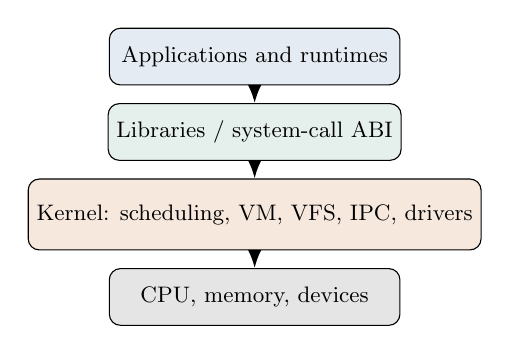
\begin{tikzpicture}[scale=.9,transform shape,node distance=2.5mm,every node/.style={font=\small,align=center}]
        \node[draw,rounded corners,fill=osblue!12,minimum width=4.1cm,minimum height=.8cm] (apps) {Applications and runtimes};
        \node[draw,rounded corners,fill=osgreen!12,minimum width=4.1cm,minimum height=.8cm,below=of apps] (api) {Libraries / system-call ABI};
        \node[draw,rounded corners,fill=osorange!15,minimum width=4.1cm,minimum height=1.0cm,below=of api] (kernel) {Kernel: scheduling, VM, VFS, IPC, drivers};
        \node[draw,rounded corners,fill=black!10,minimum width=4.1cm,minimum height=.8cm,below=of kernel] (hw) {CPU, memory, devices};
        \draw[-{Latex},thick] (apps)--(api);
        \draw[-{Latex},thick] (api)--(kernel);
        \draw[-{Latex},thick] (kernel)--(hw);
      \end{tikzpicture}
  \end{columns}
  \note{Stress that an OS is not merely a GUI or a collection of utilities. The kernel implements the privileged core; user-space services and libraries complete the usable operating environment. Ask students to classify CPU scheduling: context-switch code is mechanism, selection rule is policy.}
\end{frame}

\begin{frame}{Architecture: where should services run?}
  \small
  \begin{tabularx}{\textwidth}{@{}lXXX@{}}
    \toprule
    & \textbf{Monolithic/modular} & \textbf{Microkernel} & \textbf{Hybrid / library OS} \\
    \midrule
    Placement & Most services in kernel; loadable modules & Minimal kernel; servers in user space & Pragmatic mix or application-linked services \\
    Strength & Fast in-kernel calls; mature ecosystem & Fault isolation; small trusted core & Tunable performance/isolation balance \\
    Cost & Large privileged attack surface & IPC and crossing overhead; complex coordination & Architectural complexity; blurred boundaries \\
    Examples & Linux, BSD & seL4, QNX, MINIX 3 & Windows NT, XNU; unikernels \\
    \bottomrule
  \end{tabularx}
  \vspace{0.6em}
  \begin{tcolorbox}[title=Graduate-level lens]
    Architecture is not a binary label. Modern kernels combine modules, user-space daemons, hardware isolation, verified components, and fast shared-memory IPC. Evaluate the \emph{trusted computing base}, failure containment, and crossing cost.
  \end{tcolorbox}
  \note{Clarify that Linux is monolithic but modular, while XNU and Windows NT are commonly called hybrid. Do not imply that every microkernel system is automatically secure: the server graph, authority model, and implementation still matter.}
\end{frame}

\begin{frame}{Why historical categories are insufficient}
  \begin{columns}[T,onlytextwidth]
    \column{0.48\textwidth}
      \textbf{Workload goals}
      \begin{itemize}
        \item batch: throughput and utilization;
        \item interactive: latency and fairness;
        \item real-time: bounded worst-case response;
        \item mobile/embedded: energy, footprint, predictability;
        \item cloud: isolation, elasticity, observability.
      \end{itemize}
    \column{0.48\textwidth}
      \textbf{Modern systems are combinations}
      \begin{itemize}
        \item Linux supports batch, interactive, and real-time policies.
        \item A phone combines an application OS, secure enclave, and several RTOS-controlled devices.
        \item A cloud host combines a kernel, hypervisor features, containers, and distributed control planes.
      \end{itemize}
  \end{columns}
  \begin{alertblock}{Precision}
    An RTOS does not magically guarantee every deadline. Guarantees require schedulable workloads, bounded interrupt/blocking times, suitable policies, and analyzable hardware/software paths.
  \end{alertblock}
\end{frame}

% =============================================================================
\section{Privilege, System Calls, and Execution}
% =============================================================================

\begin{frame}{Privilege boundaries and control transfer}
  \centering
  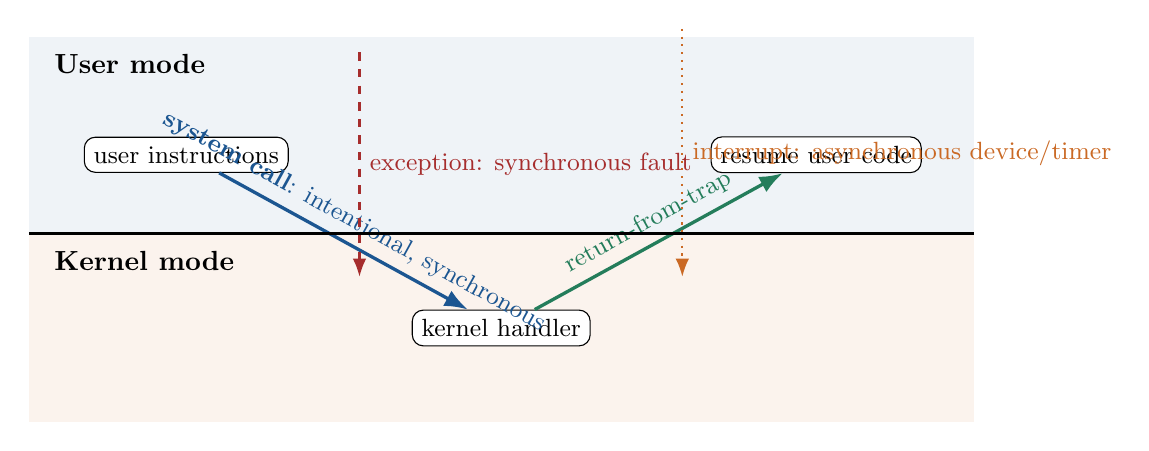
\begin{tikzpicture}[x=1cm,y=1cm,font=\small]
    \fill[osblue!7] (0,2.2) rectangle (12,4.7);
    \fill[osorange!8] (0,-0.2) rectangle (12,2.2);
    \node[anchor=west,font=\bfseries] at (.2,4.35) {User mode};
    \node[anchor=west,font=\bfseries] at (.2,1.85) {Kernel mode};
    \node[draw,rounded corners,fill=white] (u) at (2.0,3.2) {user instructions};
    \node[draw,rounded corners,fill=white] (k) at (6.0,1.0) {kernel handler};
    \node[draw,rounded corners,fill=white] (u2) at (10.0,3.2) {resume user code};
    \draw[-{Latex},very thick,osblue] (u) -- node[above,sloped]{\textbf{system call}: intentional, synchronous} (k);
    \draw[-{Latex},very thick,osgreen] (k) -- node[above,sloped]{return-from-trap} (u2);
    \draw[-{Latex},thick,dashed,osred] (4.2,4.5) -- node[right]{exception: synchronous fault} (4.2,1.65);
    \draw[-{Latex},thick,dotted,osorange] (8.3,4.8) -- node[right]{interrupt: asynchronous device/timer} (8.3,1.65);
    \draw[thick] (0,2.2)--(12,2.2);
  \end{tikzpicture}
  \begin{itemize}
    \item Hardware saves a defined architectural state, switches privilege/stack as required, and vectors to a registered handler.
    \item The kernel validates arguments and authority; a system-call number is not permission.
    \item A mode switch \alert{does not necessarily schedule another thread}.
  \end{itemize}
  \note{Correct the common misconception: syscall entry changes privilege level and execution context within the same thread. A context switch occurs only if the scheduler selects a different runnable thread. Page faults are synchronous exceptions; device interrupts are asynchronous relative to the current instruction stream.}
\end{frame}

\begin{frame}{System-call path: API, ABI, validation, result}
  \begin{columns}[T,onlytextwidth]
    \column{0.52\textwidth}
      \begin{enumerate}
        \item Application calls a library API, e.g., \code{read(fd, buf, n)}.
        \item A wrapper places the syscall number/arguments per the ABI and executes a trap instruction.
        \item Entry code switches to a protected kernel stack and dispatches the handler.
        \item Kernel checks descriptor validity, access rights, address ranges, and object state.
        \item The call completes, blocks, or returns an error; the wrapper exposes the result/\code{errno}.
      \end{enumerate}
    \column{0.45\textwidth}
      \begin{tcolorbox}[title=Three different events]
        \small
        \textbf{Mode switch}: privilege changes.\\
        \textbf{Context switch}: running thread changes.\\
        \textbf{Address-space switch}: translation context changes.
      \end{tcolorbox}
      \begin{exampleblock}{Fast paths}
        Some APIs avoid a trap: \code{vDSO} code can read kernel-published time data in user space; \code{io\_uring} amortizes crossings through shared queues and batching.
      \end{exampleblock}
  \end{columns}
\end{frame}

\begin{frame}{Process: a protected execution environment}
  \small
  \begin{columns}[T,onlytextwidth]
    \column{0.52\textwidth}
      A process is more than ``a program in execution.'' It combines:
      \begin{itemize}
        \item a virtual address space and memory mappings;
        \item one or more schedulable threads;
        \item handles/file descriptors and IPC endpoints;
        \item credentials, namespaces, limits, and accounting;
        \item signal/disposition state and parent/child relationships.
      \end{itemize}
      \begin{block}{Kernel representation}
        A process/thread control structure stores scheduling state, saved registers, kernel stack references, memory-map pointers, and resource metadata.
      \end{block}
    \column{0.44\textwidth}
      \centering
      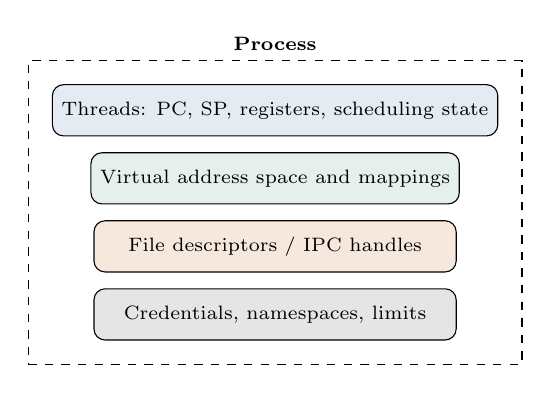
\begin{tikzpicture}[font=\scriptsize,node distance=2mm]
        \node[draw,rounded corners,fill=osblue!12,minimum width=4.6cm,minimum height=.65cm] (thr) {Threads: PC, SP, registers, scheduling state};
        \node[draw,rounded corners,fill=osgreen!12,minimum width=4.6cm,minimum height=.65cm,below=of thr] (vm) {Virtual address space and mappings};
        \node[draw,rounded corners,fill=osorange!15,minimum width=4.6cm,minimum height=.65cm,below=of vm] (fd) {File descriptors / IPC handles};
        \node[draw,rounded corners,fill=black!10,minimum width=4.6cm,minimum height=.65cm,below=of fd] (sec) {Credentials, namespaces, limits};
        \node[draw,dashed,fit=(thr)(vm)(fd)(sec),inner sep=3mm,label=above:{\bfseries Process}] {};
      \end{tikzpicture}
  \end{columns}
  \note{Different kernels model process and thread identity differently. In Linux, clone flags determine which resources tasks share; a task is the schedulable entity. Avoid presenting the PCB as one universal concrete structure.}
\end{frame}

\begin{frame}[shrink=1]{Thread state transitions}
  \small
  \centering
  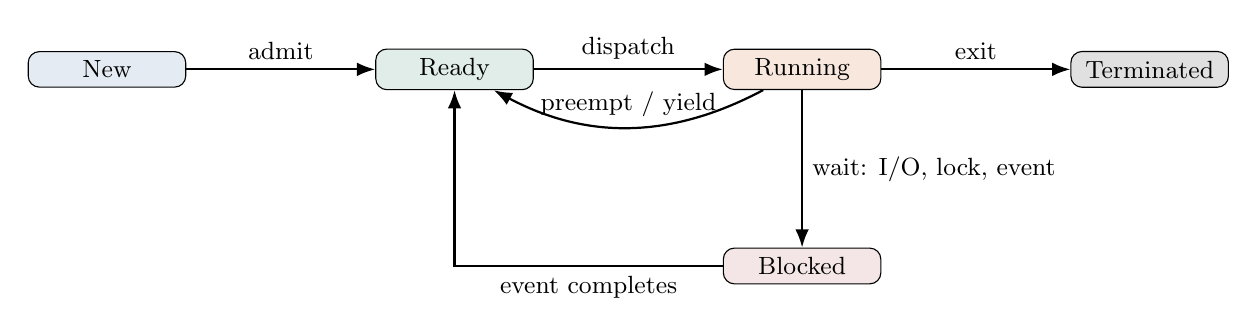
\begin{tikzpicture}[>=Latex,node distance=2.0cm and 2.4cm,font=\small]
    \node[draw,rounded corners,fill=osblue!12,minimum width=2.0cm] (new) {New};
    \node[draw,rounded corners,fill=osgreen!14,minimum width=2.0cm,right=of new] (ready) {Ready};
    \node[draw,rounded corners,fill=osorange!16,minimum width=2.0cm,right=of ready] (run) {Running};
    \node[draw,rounded corners,fill=osred!12,minimum width=2.0cm,below=of run] (block) {Blocked};
    \node[draw,rounded corners,fill=black!12,minimum width=2.0cm,right=of run] (term) {Terminated};
    \draw[->,thick] (new)--node[above]{admit}(ready);
    \draw[->,thick] (ready)--node[above]{dispatch}(run);
    \draw[->,thick,bend left=28] (run) to node[above]{preempt / yield}(ready);
    \draw[->,thick] (run)--node[right]{wait: I/O, lock, event}(block);
    \draw[->,thick] (block)-|node[pos=.25,below]{event completes}(ready);
    \draw[->,thick] (run)--node[above]{exit}(term);
  \end{tikzpicture}
  \vspace{0.5em}
  \begin{tcolorbox}[title=Important distinction]
    ``Blocked'' means not runnable until an event occurs. ``Ready'' means runnable but waiting for a CPU. A swapped-out or suspended state is an optional policy-specific refinement, not a universal base state.
  \end{tcolorbox}
\end{frame}

\begin{frame}[fragile]{Case study: launching \code{gcc file.c}}
  \small
  \begin{columns}[T,onlytextwidth]
    \column{0.47\textwidth}
\begin{lstlisting}[language=C]
pid_t pid = fork();
if (pid == 0) {
    execlp("gcc", "gcc", "file.c", NULL);
    _exit(127);              // exec failed
}
int status;
while (waitpid(pid, &status, 0) < 0 &&
       errno == EINTR) { }
\end{lstlisting}
    \column{0.50\textwidth}
      \begin{enumerate}
        \item \code{fork()} creates a child with a logically copied address space, normally implemented using \concept{copy-on-write}.
        \item \code{execve()} replaces the child's mappings and initializes a new program image; it does not create a process.
        \item The loader maps the executable/interpreter and prepares arguments, environment, stack, and entry state.
        \item \code{waitpid()} blocks the shell until child state changes, then reaps termination metadata.
      \end{enumerate}
  \end{columns}
  \begin{alertblock}{What the scheduler does}
    It schedules runnable threads throughout this sequence; scheduling is not a single stage ``after \code{exec}.'' The compiler may block repeatedly on page faults and file I/O.
  \end{alertblock}
  \note{Mention that shells may use posix_spawn, vfork, pipelines, redirection, and job-control process groups. Dynamic linking and demand paging mean the entire compiler binary need not be read before its first instruction executes.}
\end{frame}

\begin{frame}{Threads, parallelism, and multicore reality}
  \begin{columns}[T,onlytextwidth]
    \column{0.50\textwidth}
      \textbf{Threads in one process usually share}
      \begin{itemize}
        \item code, heap, memory mappings;
        \item open-file table and process credentials;
        \item failure fate: memory corruption is process-wide.
      \end{itemize}
      \textbf{Each thread retains}
      \begin{itemize}
        \item registers, program counter, stack;
        \item scheduling and signal-mask state;
        \item thread-local storage.
      \end{itemize}
    \column{0.47\textwidth}
      \begin{block}{Concurrency versus parallelism}
        \concept{Concurrency}: multiple activities overlap in time.\\
        \concept{Parallelism}: activities execute simultaneously on different processing units.
      \end{block}
      \begin{tcolorbox}[title=Multicore complications,colback=osorange!5,colframe=osorange!65]
        Cache coherence, NUMA placement, false sharing, memory ordering, interrupt affinity, and lock contention can dominate algorithmic work.
      \end{tcolorbox}
  \end{columns}
\end{frame}

\begin{frame}{Context switching: state and cost}
  \begin{columns}[T,onlytextwidth]
    \column{0.54\textwidth}
      \textbf{Potentially saved/restored}
      \begin{itemize}
        \item program counter, stack pointer, general registers, flags;
        \item floating-point/vector state, often lazily or conditionally;
        \item kernel stack and accounting/debug state;
        \item address-space identifier/page-table root when changing processes.
      \end{itemize}
    \column{0.43\textwidth}
      \textbf{Cost is not only instructions}
      \begin{itemize}
        \item hot cache lines are displaced;
        \item branch predictors and prefetch streams lose relevance;
        \item TLB effects depend on ASIDs/PCIDs and invalidations;
        \item migrations add cache/NUMA penalties.
      \end{itemize}
  \end{columns}
  \begin{tcolorbox}[title=Measurement rule]
    Avoid quoting one universal ``context-switch time.'' Measure the relevant path, workload, architecture, kernel configuration, and cache state; distinguish direct switching latency from indirect microarchitectural cost.
  \end{tcolorbox}
\end{frame}

% =============================================================================
\section{Scheduling and Real-Time Analysis}
% =============================================================================

\begin{frame}{Scheduling objectives and metrics}
  For job $i$ with arrival $a_i$, first run $s_i$, completion $c_i$, and service time $b_i$:
  \[
    \text{response } R_i=s_i-a_i,\qquad
    \text{turnaround } T_i=c_i-a_i,\qquad
    \text{waiting } W_i=T_i-b_i.
  \]
  \begin{columns}[T,onlytextwidth]
    \column{0.49\textwidth}
      \textbf{Common objectives}
      \begin{itemize}
        \item low tail latency and good responsiveness;
        \item high throughput/utilization;
        \item fairness or proportional share;
        \item deadline satisfaction and predictability.
      \end{itemize}
    \column{0.48\textwidth}
      \begin{alertblock}{No single optimum}
        Objectives conflict. Minimizing mean turnaround can starve long jobs; fairness can reduce throughput; energy-aware consolidation can increase latency.
      \end{alertblock}
  \end{columns}
  \note{Response time here means time until first service, common in introductory scheduling. In real-time analysis, response time often means release-to-completion. State the convention whenever ambiguity matters.}
\end{frame}

\begin{frame}{Classical policies and modern refinements}
  \small
  \begin{tabularx}{\textwidth}{@{}lXXX@{}}
    \toprule
    \textbf{Policy} & \textbf{Idea} & \textbf{Strength} & \textbf{Failure mode / refinement} \\
    \midrule
    FCFS & arrival order & simple, low overhead & convoy effect \\
    SJF/SRTF & shortest predicted work & minimizes mean completion time under assumptions & future burst unknown; starvation \\
    Round robin & rotating time quantum & responsive, bounded turn wait & too-small quantum raises overhead \\
    Priority & highest priority first & expresses importance & starvation; aging; inversion handling \\
    Fair-share & allocate weighted CPU share & multi-tenant fairness & latency depends on runnable population \\
    Multilevel feedback & infer behavior from history & adapts to interactive/CPU-bound tasks & gaming and tuning complexity \\
    \bottomrule
  \end{tabularx}
  \smallnote{Production schedulers also account for multicore load balancing, affinity, topology, energy, bandwidth contention, and heterogeneous CPUs.}
\end{frame}

\begin{frame}{Real-time scheduling: guarantees require analysis}
  For periodic task $\tau_i=(C_i,T_i,D_i)$, $C_i$ is worst-case execution time, $T_i$ period, and $D_i$ relative deadline.
  \begin{columns}[T,onlytextwidth]
    \column{0.53\textwidth}
      \begin{block}{Utilization}
        \[
          U=\sum_{i=1}^{n}\frac{C_i}{T_i}.
        \]
        On one preemptive CPU with independent tasks and $D_i=T_i$, earliest-deadline-first is schedulable if $U\leq 1$ under the ideal model.
      \end{block}
    \column{0.44\textwidth}
      \textbf{Reality adds}
      \begin{itemize}
        \item blocking and non-preemptive regions;
        \item interrupt and kernel interference;
        \item cache/bus contention and execution-time variation;
        \item release jitter, overload, and multicore complications.
      \end{itemize}
  \end{columns}
  \begin{alertblock}{Hard versus soft real time}
    ``Hard'' means a missed deadline is unacceptable by specification; ``soft'' means lateness degrades utility. It does not mean ``fast'' versus ``slow.''
  \end{alertblock}
  \note{The EDF utilization statement relies on the standard uniprocessor model. For fixed-priority rate-monotonic scheduling, the classic sufficient bound is n(2^(1/n)-1), approaching ln 2, but exact response-time analysis is stronger.}
\end{frame}

\begin{frame}{Priority inversion and bounded blocking}
  \centering
  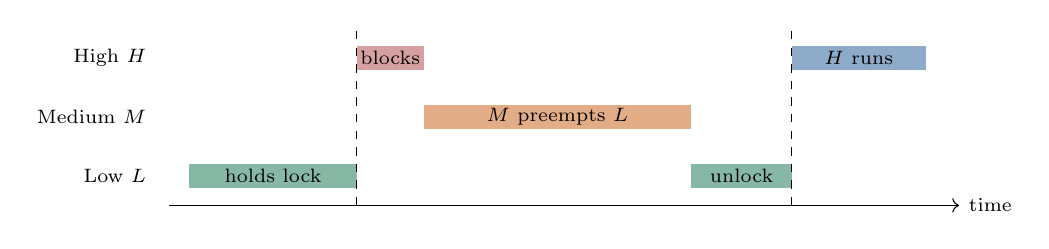
\begin{tikzpicture}[x=.85cm,y=.75cm,font=\scriptsize]
    \node[anchor=east] at (0,3) {High $H$};
    \node[anchor=east] at (0,2) {Medium $M$};
    \node[anchor=east] at (0,1) {Low $L$};
    \draw[->] (0.2,.5)--(12,.5) node[right]{time};
    \fill[osgreen!55] (.5,.8) rectangle (3,1.2);
    \node at (1.75,1) {holds lock};
    \fill[osred!45] (3,2.8) rectangle (4,3.2);
    \node at (3.5,3) {blocks};
    \fill[osorange!55] (4,1.8) rectangle (8,2.2);
    \node at (6,2) {$M$ preempts $L$};
    \fill[osgreen!55] (8,.8) rectangle (9.5,1.2);
    \node at (8.75,1) {unlock};
    \fill[osblue!50] (9.5,2.8) rectangle (11.5,3.2);
    \node at (10.5,3) {$H$ runs};
    \draw[dashed] (3,.5)--(3,3.5);
    \draw[dashed] (9.5,.5)--(9.5,3.5);
  \end{tikzpicture}
  \begin{itemize}
    \item A high-priority thread waits for a lock held by a low-priority thread, while medium-priority work delays the lock holder.
    \item \concept{Priority inheritance} temporarily raises the owner's effective priority; \concept{priority-ceiling protocols} can provide analyzable blocking bounds.
  \end{itemize}
\end{frame}

% =============================================================================
\section{Synchronization and Concurrency}
% =============================================================================

\begin{frame}[fragile]{Race conditions and atomicity}
  \small
  \begin{columns}[T,onlytextwidth]
    \column{0.47\textwidth}
\begin{lstlisting}[language=C]
// Incorrect if multiple threads execute it
counter++;

// Conceptual expansion
r = load(counter);
r = r + 1;
store(counter, r);
\end{lstlisting}
    \column{0.50\textwidth}
      A \concept{data race} occurs when conflicting accesses to the same location are concurrent, at least one is a write, and synchronization does not order them.
      \begin{itemize}
        \item Atomicity prevents torn/interleaved operations.
        \item Ordering determines which effects may be observed.
        \item Visibility requires communication through the memory model.
      \end{itemize}
      \begin{alertblock}{C/C++ caveat}
        A data race on a non-atomic object yields undefined behavior; ``it works on my CPU'' is not a correctness argument.
      \end{alertblock}
  \end{columns}
  \note{Separate race condition, a broader logic error dependent on timing, from the language-level definition of a data race. Compiler reordering matters in addition to CPU reordering. Volatile is not a substitute for atomics or locks in C/C++.}
\end{frame}

\begin{frame}{Happens-before: the useful abstraction}
  \begin{columns}[T,onlytextwidth]
    \column{0.55\textwidth}
      \begin{block}{Reasoning rule}
        If event $A$ \concept{happens-before} event $B$, then $B$ must observe the effects of $A$ required by the language/OS synchronization semantics.
      \end{block}
      Typical ordering edges include:
      \begin{itemize}
        \item program order within one thread;
        \item mutex unlock $\rightarrow$ later successful lock;
        \item thread creation and join;
        \item release/acquire operations on compatible atomics.
      \end{itemize}
    \column{0.42\textwidth}
      \centering
      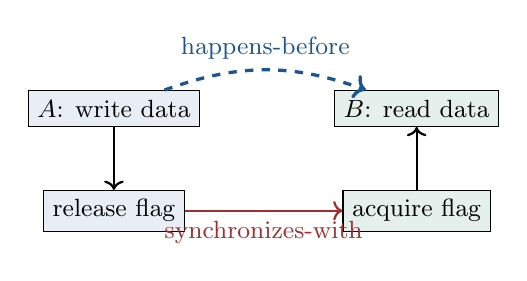
\begin{tikzpicture}[font=\small,node distance=8mm]
        \node[draw,fill=osblue!10] (wa) {$A$: write data};
        \node[draw,fill=osblue!10,below=of wa] (rel) {release flag};
        \node[draw,fill=osgreen!12,right=2cm of rel] (acq) {acquire flag};
        \node[draw,fill=osgreen!12,above=of acq] (rb) {$B$: read data};
        \draw[->,thick] (wa)--(rel);
        \draw[->,thick,osred] (rel)--node[below]{synchronizes-with}(acq);
        \draw[->,thick] (acq)--(rb);
        \draw[->,very thick,dashed,osblue,bend left=20] (wa) to node[above]{happens-before}(rb);
      \end{tikzpicture}
  \end{columns}
\end{frame}

\begin{frame}[fragile]{Condition variables: wait in a loop}
\begin{lstlisting}[language=C]
pthread_mutex_lock(&m);
while (queue_empty(&q)) {          // predicate, not an event count
    pthread_cond_wait(&not_empty, &m);
    // atomically releases m while sleeping, then reacquires m
}
item = queue_pop(&q);
pthread_mutex_unlock(&m);
\end{lstlisting}
  \begin{columns}[T,onlytextwidth]
    \column{0.49\textwidth}
      \textbf{Why the loop?}
      \begin{itemize}
        \item wakeups may be spurious;
        \item another consumer may win the race;
        \item the predicate can become false before reacquisition.
      \end{itemize}
    \column{0.48\textwidth}
      \textbf{Lock design}
      \begin{itemize}
        \item keep invariants explicit;
        \item avoid blocking I/O while holding a lock;
        \item choose granularity using contention measurements;
        \item prefer structured ownership where possible.
      \end{itemize}
  \end{columns}
\end{frame}

\begin{frame}{Advanced synchronization toolbox}
  \scriptsize
  \begin{tabularx}{\textwidth}{@{}lXX@{}}
    \toprule
    \textbf{Primitive} & \textbf{Use} & \textbf{Key risk / insight} \\
    \midrule
    Mutex & exclusive access to an invariant & contention, convoying, priority inversion \\
    Semaphore & counting resources or signaling & ownership is weaker; easy to mis-pair operations \\
    Read--write lock & read-dominant shared state & writer starvation; overhead can exceed a mutex \\
    Seqlock & many readers, rare short writes & readers retry; unsuitable for pointer reclamation alone \\
    RCU & read-mostly structures & reclamation waits for grace periods; complex update semantics \\
    Futex & user-space fast path, kernel-assisted sleep & basis for many Linux locks, not a policy itself \\
    Lock-free atomics & system-wide progress despite a stalled thread & ABA, reclamation, memory-order complexity \\
    \bottomrule
  \end{tabularx}
  \begin{tcolorbox}[title=Engineering principle]
    ``Lock-free'' is not synonymous with wait-free, faster, simpler, or starvation-free. State the progress guarantee and prove memory safety as well as atomic correctness.
  \end{tcolorbox}
\end{frame}

\begin{frame}{Deadlock: conditions, graph, and strategies}
  \begin{columns}[T,onlytextwidth]
    \column{0.47\textwidth}
      Four necessary Coffman conditions:
      \begin{enumerate}
        \item mutual exclusion;
        \item hold and wait;
        \item no forced preemption;
        \item circular wait.
      \end{enumerate}
      \begin{block}{Design responses}
        Prevent one condition, avoid unsafe states, detect and recover, or accept the risk when justified.
      \end{block}
    \column{0.50\textwidth}
      \centering
      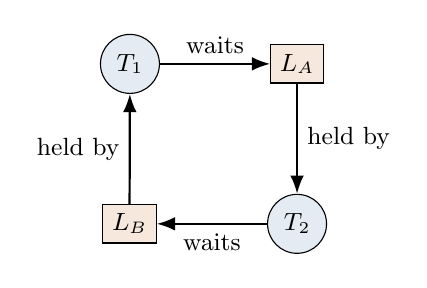
\begin{tikzpicture}[>=Latex,font=\small,node distance=1.4cm]
        \node[draw,circle,fill=osblue!12] (t1) {$T_1$};
        \node[draw,rectangle,fill=osorange!15,right=of t1] (a) {$L_A$};
        \node[draw,circle,fill=osblue!12,below=of a] (t2) {$T_2$};
        \node[draw,rectangle,fill=osorange!15,left=of t2] (b) {$L_B$};
        \draw[->,thick] (t1)--node[above]{waits}(a);
        \draw[->,thick] (a)--node[right]{held by}(t2);
        \draw[->,thick] (t2)--node[below]{waits}(b);
        \draw[->,thick] (b)--node[left]{held by}(t1);
      \end{tikzpicture}
      \smallnote{A cycle implies deadlock for single-instance resources; with multiple instances, a cycle is necessary but not always sufficient.}
  \end{columns}
\end{frame}

% =============================================================================
\section{Virtual Memory and Memory Management}
% =============================================================================

\begin{frame}{Virtual address space: isolation plus indirection}
  \small
  \begin{columns}[T,onlytextwidth]
    \column{0.43\textwidth}
      \centering
      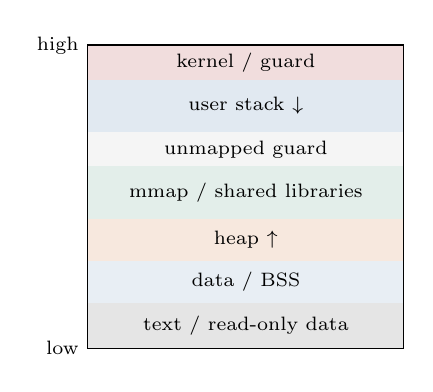
\begin{tikzpicture}[y=.48cm,font=\scriptsize]
        \draw[thick] (0,0) rectangle (4,8);
        \fill[osred!16] (0,7.1) rectangle (4,8); \node at (2,7.55) {kernel / guard};
        \fill[osblue!13] (0,5.7) rectangle (4,7.1); \node at (2,6.4) {user stack $\downarrow$};
        \fill[black!4] (0,4.8) rectangle (4,5.7); \node at (2,5.25) {unmapped guard};
        \fill[osgreen!13] (0,3.4) rectangle (4,4.8); \node at (2,4.1) {mmap / shared libraries};
        \fill[osorange!15] (0,2.3) rectangle (4,3.4); \node at (2,2.85) {heap $\uparrow$};
        \fill[osblue!10] (0,1.2) rectangle (4,2.3); \node at (2,1.75) {data / BSS};
        \fill[black!10] (0,0) rectangle (4,1.2); \node at (2,.6) {text / read-only data};
        \node[left] at (0,0) {low};
        \node[left] at (0,8) {high};
      \end{tikzpicture}
    \column{0.54\textwidth}
      \begin{itemize}
        \item Every process sees a private, sparse virtual address space; mappings need not occupy contiguous physical frames.
        \item Page permissions enforce read/write/execute and user/kernel access.
        \item Shared mappings permit efficient IPC and shared libraries.
        \item ASLR randomizes placement; guard pages turn some overflows into faults.
        \item The diagram is conceptual: exact layout depends on ABI, architecture, loader, and policy.
      \end{itemize}
      \smallnote{Virtual memory supplies protection and placement. Demand paging is a common policy layered on top.}
  \end{columns}
  \note{Avoid claiming that the whole kernel is necessarily mapped into every process; mitigations and architectures differ. The stack/heap direction is conventional, not guaranteed by the virtual-memory abstraction.}
\end{frame}

\begin{frame}{Address translation and the TLB}
  \centering
  \resizebox{0.94\textwidth}{!}{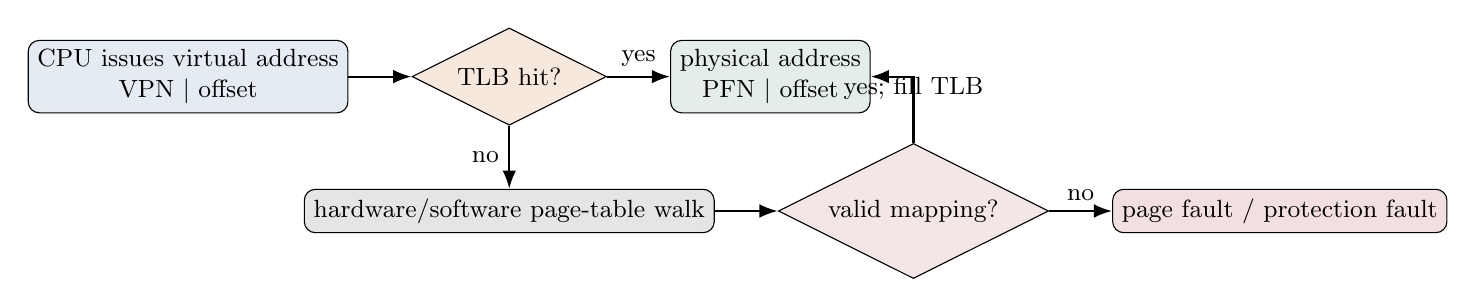
\begin{tikzpicture}[>=Latex,font=\small,node distance=8mm,every node/.style={align=center}]
    \node[draw,rounded corners,fill=osblue!12] (cpu) {CPU issues virtual address\\VPN $\mid$ offset};
    \node[draw,diamond,aspect=2,fill=osorange!15,right=of cpu] (tlb) {TLB hit?};
    \node[draw,rounded corners,fill=osgreen!13,right=of tlb] (pa) {physical address\\PFN $\mid$ offset};
    \node[draw,rounded corners,fill=black!10,below=of tlb] (walk) {hardware/software page-table walk};
    \node[draw,diamond,aspect=2,fill=osred!12,right=of walk] (valid) {valid mapping?};
    \node[draw,rounded corners,fill=osred!15,right=of valid] (fault) {page fault / protection fault};
    \draw[->,thick] (cpu)--(tlb);
    \draw[->,thick] (tlb)--node[above]{yes}(pa);
    \draw[->,thick] (tlb)--node[left]{no}(walk);
    \draw[->,thick] (walk)--(valid);
    \draw[->,thick] (valid)|-node[pos=.25,above]{yes; fill TLB}(pa);
    \draw[->,thick] (valid)--node[above]{no}(fault);
  \end{tikzpicture}}
  \begin{itemize}
    \item Multi-level page tables make sparse spaces practical; huge pages reduce TLB pressure but increase internal fragmentation and migration cost.
    \item A TLB miss is normally resolved by a page-table walk; it is \alert{not automatically a page fault}.
  \end{itemize}
\end{frame}

\begin{frame}{Page faults: minor, major, and protection}
  \begin{enumerate}
    \item CPU detects a missing or disallowed translation and traps to the kernel.
    \item Kernel locates the virtual-memory area and checks requested access.
    \item If valid, it may allocate a zero page, resolve copy-on-write, or fetch file/swap data.
    \item Page tables and relevant TLB entries are updated; the faulting instruction restarts.
  \end{enumerate}
  \begin{columns}[T,onlytextwidth]
    \column{0.32\textwidth}
      \begin{block}{Minor fault}
        No storage I/O required; mapping/data is already resident or can be created cheaply.
      \end{block}
    \column{0.32\textwidth}
      \begin{block}{Major fault}
        Requires storage I/O and can be orders of magnitude slower.
      \end{block}
    \column{0.32\textwidth}
      \begin{alertblock}{Invalid access}
        Kernel cannot resolve it; the process receives a fault signal/exception or is terminated.
      \end{alertblock}
  \end{columns}
\end{frame}

\begin{frame}{Copy-on-write makes \code{fork()} practical}
  \begin{columns}[T,onlytextwidth]
    \column{0.48\textwidth}
      \textbf{Immediately after \code{fork()}}
      \begin{itemize}
        \item parent and child mappings reference the same physical frames;
        \item writable pages are marked read-only/COW;
        \item reference counts track sharing.
      \end{itemize}
      \textbf{On a write fault}
      \begin{itemize}
        \item allocate a new frame;
        \item copy the old contents;
        \item remap the writer's page as writable.
      \end{itemize}
    \column{0.49\textwidth}
      \centering
      \resizebox{\linewidth}{!}{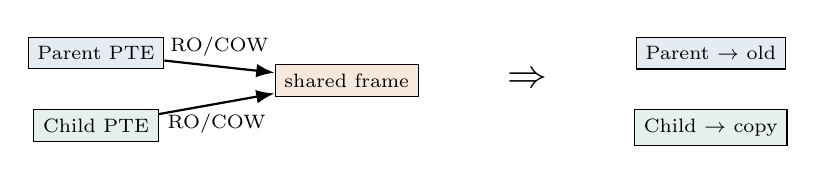
\begin{tikzpicture}[>=Latex,font=\scriptsize,node distance=5mm]
        \node[draw,fill=osblue!12] (p1) {Parent PTE};
        \node[draw,fill=osgreen!12,below=of p1] (c1) {Child PTE};
        \node[draw,fill=osorange!15,right=1.4cm of p1,yshift=-.35cm] (f1) {shared frame};
        \draw[->,thick] (p1)--node[above]{RO/COW}(f1);
        \draw[->,thick] (c1)--node[below]{RO/COW}(f1);
        \node[right=1.0cm of f1,font=\Large] (arr) {$\Rightarrow$};
        \node[draw,fill=osblue!12,right=1.0cm of arr,yshift=.35cm] (p2) {Parent $\to$ old};
        \node[draw,fill=osgreen!12,below=of p2] (c2) {Child $\to$ copy};
      \end{tikzpicture}}
      \smallnote{If the child quickly calls \code{execve()}, most pages are never copied. Page-table copying and shootdowns can still be significant for very large processes.}
  \end{columns}
\end{frame}

\begin{frame}{Memory pressure, replacement, and NUMA}
  \begin{columns}[T,onlytextwidth]
    \column{0.49\textwidth}
      \textbf{Replacement goals}
      \begin{itemize}
        \item approximate recency/frequency without exact LRU cost;
        \item balance anonymous and file-backed pages;
        \item preserve a workload's working set;
        \item write back dirty pages without bursty stalls.
      \end{itemize}
      \begin{alertblock}{Thrashing}
        If active working sets exceed available memory, page-fault work can dominate useful execution. Adding runnable jobs may reduce throughput.
      \end{alertblock}
    \column{0.47\textwidth}
      \textbf{NUMA-aware management}
      \begin{itemize}
        \item local memory usually has lower latency/higher bandwidth;
        \item first-touch placement links allocation to the accessing CPU;
        \item migration trades locality benefit against movement cost;
        \item CPU affinity and memory placement must be considered together.
      \end{itemize}
      \begin{tcolorbox}[title=Modern concern,colback=osorange!5,colframe=osorange!65]
        Memory bandwidth and cache capacity can be the scarce resources even when free pages and CPU time remain.
      \end{tcolorbox}
  \end{columns}
\end{frame}

% =============================================================================
\section{Storage and Distributed Filesystems}
% =============================================================================

\begin{frame}{From \code{read()} to persistent storage}
  \centering
  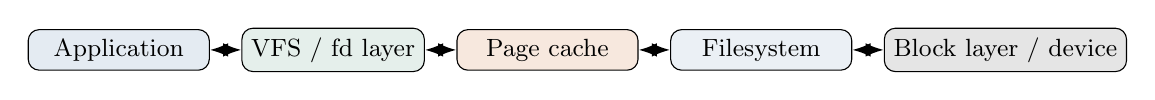
\begin{tikzpicture}[>=Latex,font=\small,node distance=4mm]
    \node[draw,rounded corners,fill=osblue!12,minimum width=2.3cm] (app) {Application};
    \node[draw,rounded corners,fill=osgreen!12,minimum width=2.3cm,right=of app] (vfs) {VFS / fd layer};
    \node[draw,rounded corners,fill=osorange!15,minimum width=2.3cm,right=of vfs] (cache) {Page cache};
    \node[draw,rounded corners,fill=osblue!9,minimum width=2.3cm,right=of cache] (fs) {Filesystem};
    \node[draw,rounded corners,fill=black!10,minimum width=2.3cm,right=of fs] (dev) {Block layer / device};
    \draw[<->,thick] (app)--(vfs);
    \draw[<->,thick] (vfs)--(cache);
    \draw[<->,thick] (cache)--(fs);
    \draw[<->,thick] (fs)--(dev);
  \end{tikzpicture}
  \begin{columns}[T,onlytextwidth]
    \column{0.49\textwidth}
      \begin{itemize}
        \item VFS provides a common namespace/object interface.
        \item The page cache unifies many buffered reads and memory-mapped file pages.
        \item Read-ahead and write-back convert application access into efficient I/O.
      \end{itemize}
    \column{0.48\textwidth}
      \begin{itemize}
        \item \code{write()} returning does not generally imply durable media persistence.
        \item Durability requires defined APIs such as \code{fsync()} plus correct device/cache behavior.
        \item Direct I/O bypasses parts of caching but adds alignment and coordination constraints.
      \end{itemize}
  \end{columns}
\end{frame}

\begin{frame}{Crash consistency: preserving invariants}
  A crash can expose only a prefix or reordering of intended writes. The filesystem must prevent metadata/data structures from becoming inconsistent.
  \begin{columns}[T,onlytextwidth]
    \column{0.31\textwidth}
      \begin{block}{Journaling / WAL}
        Record intended updates in a log, commit them, then checkpoint to home locations.
      \end{block}
    \column{0.31\textwidth}
      \begin{block}{Copy-on-write}
        Write new blocks and atomically redirect a root/reference; retain old reachable state.
      \end{block}
    \column{0.31\textwidth}
      \begin{block}{Log-structured}
        Append updates sequentially; recover from checkpoints and log scanning.
      \end{block}
  \end{columns}
  \begin{alertblock}{Durability is end-to-end}
    Application update protocol, filesystem ordering, storage barriers, controller caches, and device semantics must agree. Atomic rename alone does not automatically make every multi-file transaction durable.
  \end{alertblock}
\end{frame}

\begin{frame}{Distributed filesystems: semantics under failure}
  \begin{columns}[T,onlytextwidth]
    \column{0.52\textwidth}
      Design questions:
      \begin{itemize}
        \item Who owns metadata and namespace coordination?
        \item Are reads/writes linearizable, close-to-open, session-consistent, or eventually consistent?
        \item How are blocks replicated or erasure-coded?
        \item What happens during partitions, retries, duplicate RPCs, and client failure?
        \item How are leases, locks, caching, and recovery coordinated?
      \end{itemize}
    \column{0.45\textwidth}
      \begin{tcolorbox}[title=Failure-aware API]
        A timeout means ``the client did not learn the result,'' not necessarily ``the operation did not occur.'' Operations and retry protocols should be idempotent or carry unique request identities.
      \end{tcolorbox}
      \begin{block}{Different targets}
        NFS-style sharing, parallel HPC filesystems, cloud object stores, and database storage expose different consistency and performance contracts.
      \end{block}
  \end{columns}
  \note{Use this slide to connect OS-level naming and caching to distributed systems. CAP is often oversimplified: during a network partition, a system cannot provide both availability for every request and linearizable consistency. Latency and normal-operation trade-offs also matter.}
\end{frame}

% =============================================================================
\section{Isolation, Containers, and Virtual Machines}
% =============================================================================

\begin{frame}{Containers are constrained processes, not tiny VMs}
  \begin{columns}[T,onlytextwidth]
    \column{0.50\textwidth}
      \begin{itemize}
        \item \concept{Namespaces} virtualize views of process IDs, mounts, networking, users, IPC, and host identity.
        \item \concept{cgroups} account for and limit CPU, memory, I/O, and process counts.
        \item \concept{Capabilities}, seccomp, LSMs, and filesystem permissions reduce authority.
        \item Layered images and runtimes package a user-space environment; all containers still share the host kernel.
      \end{itemize}
    \column{0.47\textwidth}
      \centering
      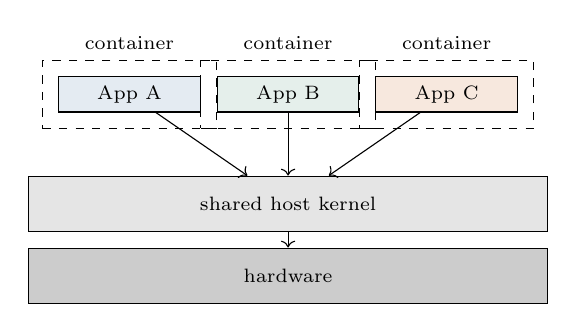
\begin{tikzpicture}[font=\scriptsize,node distance=2mm]
        \node[draw,fill=osblue!12,minimum width=1.8cm] (a1) {App A};
        \node[draw,fill=osgreen!12,minimum width=1.8cm,right=of a1] (a2) {App B};
        \node[draw,fill=osorange!15,minimum width=1.8cm,right=of a2] (a3) {App C};
        \node[draw,dashed,fit=(a1),inner sep=2mm,label=above:{container}] {};
        \node[draw,dashed,fit=(a2),inner sep=2mm,label=above:{container}] {};
        \node[draw,dashed,fit=(a3),inner sep=2mm,label=above:{container}] {};
        \node[draw,fill=black!10,minimum width=6.6cm,minimum height=.7cm,below=8mm of a2] (k) {shared host kernel};
        \node[draw,fill=black!20,minimum width=6.6cm,minimum height=.7cm,below=of k] (h) {hardware};
        \draw[->] (a1)--(k); \draw[->] (a2)--(k); \draw[->] (a3)--(k); \draw[->] (k)--(h);
      \end{tikzpicture}
      \begin{alertblock}{Security boundary}
        Container isolation depends critically on the shared kernel and configuration; use stronger isolation where the threat model requires it.
      \end{alertblock}
  \end{columns}
\end{frame}

\begin{frame}{Containers versus virtual machines}
  \small
  \begin{tabularx}{\textwidth}{@{}lXX@{}}
    \toprule
    & \textbf{Container} & \textbf{Virtual machine} \\
    \midrule
    Isolation layer & kernel objects/views and resource controls & virtual hardware plus guest kernel \\
    Kernel & shared with host & separate guest kernel \\
    Startup/footprint & usually small and fast & usually larger; snapshots can reduce startup \\
    Compatibility & host kernel ABI required & can run a different compatible guest OS/ABI \\
    Failure/security boundary & host kernel is common dependency & hypervisor/hardware boundary; still not absolute \\
    Typical use & deployment density, reproducibility & stronger tenant separation, legacy OS, kernel control \\
    \bottomrule
  \end{tabularx}
  \begin{tcolorbox}[title=Modern continuum]
    Sandboxed runtimes, microVMs, confidential VMs, and hardware enclaves combine techniques. Choose based on threat model, performance, compatibility, and operational cost.
  \end{tcolorbox}
\end{frame}

\begin{frame}{Security: mediation, least privilege, defense in depth}
  \begin{columns}[T,onlytextwidth]
    \column{0.49\textwidth}
      \textbf{Enforcement mechanisms}
      \begin{itemize}
        \item privilege levels and page permissions;
        \item identities, ACLs, capabilities, and labels;
        \item syscall filtering and sandboxing;
        \item code signing, secure boot, measured boot;
        \item audit logs and anomaly detection.
      \end{itemize}
    \column{0.48\textwidth}
      \textbf{Principles}
      \begin{itemize}
        \item least privilege and least authority;
        \item complete mediation;
        \item minimize trusted computing base;
        \item fail safely and separate duties;
        \item assume components will be compromised.
      \end{itemize}
  \end{columns}
  \begin{alertblock}{Side channels cross abstractions}
    Timing, caches, predictors, speculative execution, and shared resource contention can leak information even when architectural access checks are correct.
  \end{alertblock}
\end{frame}

% =============================================================================
\section{Diagnosis and Synthesis}
% =============================================================================

\begin{frame}{End-to-end execution: one request, many subsystems}
  \centering
  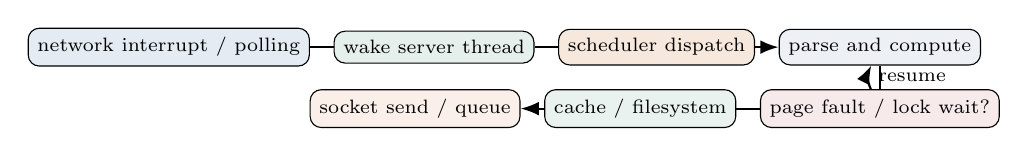
\begin{tikzpicture}[>=Latex,font=\scriptsize,node distance=3mm]
    \node[draw,rounded corners,fill=osblue!12] (req) {network interrupt / polling};
    \node[draw,rounded corners,fill=osgreen!12,right=of req] (wake) {wake server thread};
    \node[draw,rounded corners,fill=osorange!15,right=of wake] (sched) {scheduler dispatch};
    \node[draw,rounded corners,fill=osblue!8,right=of sched] (work) {parse and compute};
    \node[draw,rounded corners,fill=osred!10,below=of work] (fault) {page fault / lock wait?};
    \node[draw,rounded corners,fill=osgreen!10,left=of fault] (fs) {cache / filesystem};
    \node[draw,rounded corners,fill=osorange!10,left=of fs] (reply) {socket send / queue};
    \draw[->,thick] (req)--(wake)--(sched)--(work);
    \draw[->,thick] (work)--(fault)--(fs)--(reply);
    \draw[->,thick,dashed,bend left=25] (fault) to node[right]{resume}(work);
  \end{tikzpicture}
  \begin{tcolorbox}[title=Tail-latency lesson]
    A slow request may reflect scheduling delay, lock contention, reclaim, major faults, write-back, network queues, or device latency. Optimize only after identifying the dominant queue and causal path.
  \end{tcolorbox}
  \begin{itemize}
    \item Use traces for sequence/causality, profiles for where CPU time goes, and counters for rates/capacity symptoms.
    \item Coordinate IDs and timestamps across layers; averages often hide the failures users experience.
  \end{itemize}
\end{frame}

\begin{frame}{Common misconceptions: corrected}
  \small
  \begin{tabularx}{\textwidth}{@{}X@{\quad$\Rightarrow$\quad}X@{}}
    \toprule
    \textbf{Misconception} & \textbf{Precise statement} \\
    \midrule
    Every syscall causes a context switch. & A syscall changes privilege; another thread runs only if scheduling occurs. \\
    \code{fork()} immediately copies all memory. & It exposes copy semantics, usually via copy-on-write mappings. \\
    A TLB miss is a page fault. & A valid page-table walk can resolve a TLB miss without a fault. \\
    \code{write()} means data is durable. & It often means data reached kernel buffers; durability needs an explicit protocol. \\
    Volatile makes shared variables thread-safe. & Language atomics or synchronization establish atomicity and ordering. \\
    Containers each contain a kernel. & Ordinary containers share the host kernel; VMs run guest kernels. \\
    RTOS means all deadlines are guaranteed. & Guarantees depend on workload assumptions and schedulability analysis. \\
    \bottomrule
  \end{tabularx}
\end{frame}

\begin{frame}{Synthesis: the recurring design tensions}
  \begin{columns}[T,onlytextwidth]
    \column{0.32\textwidth}
      \begin{block}{Performance}
        Cache locality, batching, fewer crossings, asynchronous I/O, scalable synchronization.
      \end{block}
    \column{0.32\textwidth}
      \begin{block}{Correctness}
        Invariants, atomicity, ordering, bounded blocking, crash consistency, explicit semantics.
      \end{block}
    \column{0.32\textwidth}
      \begin{block}{Isolation}
        Least privilege, resource controls, fault containment, auditable trusted components.
      \end{block}
  \end{columns}
  \vspace{0.5em}
  \begin{tcolorbox}[title=Transferable method,colback=osgreen!5,colframe=osgreen!65]
    For any OS feature, ask: What abstraction is promised? Which mechanisms implement it? Which policies choose among alternatives? What assumptions can fail? How will we measure the result?
  \end{tcolorbox}
\end{frame}

\begin{frame}{Discussion and next steps}
  \begin{enumerate}
    \item Where should a database rely on the OS, and where should it bypass or specialize OS mechanisms?
    \item Which shared resource is most likely to violate isolation in a multi-tenant service: CPU time, cache, memory bandwidth, storage, or network queues?
    \item When is a stronger boundary (microVM/VM) worth its additional operational cost?
  \end{enumerate}
  \begin{block}{Suggested laboratory}
    Trace a small program using \code{strace}; inspect mappings with \code{/proc/<pid>/maps}; measure faults and switches with \code{perf stat}; then explain observed events using the models in this deck.
  \end{block}
\end{frame}

% =============================================================================
\appendix
\section{Appendix}
% =============================================================================

\begin{frame}{Knowledge check}
  \begin{enumerate}
    \item A thread calls \code{getpid()} through a vDSO implementation. Must it enter kernel mode?
    \item A TLB lookup misses, but the page-table entry is present and accessible. Is this a page fault?
    \item Why can \code{fork()} still be expensive for a process that immediately calls \code{execve()}?
    \item Give one execution in which \code{if (empty) wait()} loses a wakeup or consumes invalid state.
    \item What extra assumptions are needed before $U\leq1$ establishes EDF schedulability?
    \item After a distributed filesystem RPC times out, why is blind retry unsafe for a non-idempotent operation?
  \end{enumerate}
  \note{Answers: (1) not necessarily; vDSO can remain in user mode. (2) no, a page-table walk refills the TLB. (3) page-table duplication, metadata work, TLB effects, and very large mappings. (4) check and sleep are not atomic, or another consumer wins; use a mutex and condition loop. (5) standard independent periodic/sporadic uniprocessor assumptions, preemption, D=T, bounded/known C, and excluded or modeled overhead/blocking. (6) the operation may have committed even though its response was lost.}
\end{frame}

\begin{frame}{Exercise: analyze a deadline miss}
  A control task $H$ with period/deadline $10$ ms and WCET $2$ ms shares a mutex with a logging task $L$. A telemetry task $M$ can run for $6$ ms. At $t=0$, $L$ holds the mutex; $H$ releases and blocks; then $M$ preempts $L$.
  \begin{enumerate}
    \item Draw the schedule without priority inheritance.
    \item Identify direct blocking and interference.
    \item Redraw it with priority inheritance.
    \item What additional quantities are needed for a valid worst-case response-time bound?
  \end{enumerate}
  \begin{tcolorbox}[title=Extension]
    Compare priority inheritance with a priority-ceiling protocol. Which better supports offline blocking analysis, and what implementation constraints follow?
  \end{tcolorbox}
\end{frame}

\begin{frame}[fragile]{Exercise: diagnose the concurrent queue}
\begin{lstlisting}[language=C]
if (queue_empty(&q))
    pthread_cond_wait(&not_empty, &m);
item = queue_pop(&q);
\end{lstlisting}
  \begin{enumerate}
    \item List every precondition the fragment silently assumes.
    \item Construct an execution with two consumers that violates safety.
    \item Repair the code and state the invariant protected by \code{m}.
    \item Decide whether \code{signal} or \code{broadcast} is appropriate and justify the liveness/performance trade-off.
  \end{enumerate}
\end{frame}

\begin{frame}{Further study}
  \begin{itemize}
    \item Process/kernel interfaces: system-call ABI, signals, IPC, asynchronous I/O.
    \item Scheduling: multiprocessor fairness, deadline scheduling, energy-aware scheduling.
    \item Concurrency: memory models, RCU, lock-free reclamation, formal verification.
    \item Memory: huge pages, NUMA balancing, compressed memory, persistent memory.
    \item Storage: transactions, checksums, snapshots, replication, consensus-backed metadata.
    \item Isolation: capabilities, verified kernels, confidential computing, side-channel defenses.
  \end{itemize}
  \begin{center}
    \Large Questions?
  \end{center}
\end{frame}

\end{document}

